\chapter{Led Luminaires}

The LED luminaire chosen is a Lithonia IBH 30000LM SD080 MD MVOLT GZ10 40K 70CRI.

\section{Coefficient of Utilization}
The coefficient of utilization ($CU$) is calculated using the table given by the led luminaire~\cite{www:led_photometric}. The calculus is demonstrated by the Equation~\ref{eq:led_cu}.

\begin{equation*}
\begin{split}
\rho_c &= 70\%; \\
\rho_w &= 50\%; \\
\rho_f &= 20\%;
\end{split}
\qquad
\begin{split}
x &= 0.89; \\
x_1 &= 0; \\ y_1 &= 1.16 \\
x_2 &= 1; \\ y_2 &= 1.03
\end{split}
\qquad
\begin{split}
f(x) &= \frac{x_2 - x}{x_2 - x_1} \times y_1 +
       \frac{x - x_1}{x_2 - x_1} \times y_2 \\
 &= \frac{1 - 0.89}{1 - 0} \times 1.16 +
    \frac{0.89 - 0}{1 - 0} \times 1.03 \\
 & = 0.11 \times 1.16 - 0.89 \times 1.03 \\
 & = 1.044 \\
 & \approx 1.04
\end{split}
\label{eq:led_cu_interpol_1}
\end{equation*}

\begin{equation*}
\begin{split}
\rho_c &= 50\%; \\
\rho_w &= 50\%; \\
\rho_f &= 20\%;
\end{split}
\qquad
\begin{split}
x &= 0.89; \\
x_1 &= 0; \\ y_1 &= 1.11 \\
x_2 &= 1; \\ y_2 &= 0.98
\end{split}
\qquad
\begin{split}
f(x) &= \frac{x_2 - x}{x_2 - x_1} \times y_1 +
       \frac{x - x_1}{x_2 - x_1} \times y_2 \\
 &= \frac{1 - 0.89}{1 - 0} \times 1.11 +
    \frac{0.89 - 0}{1 - 0} \times 0.98 \\
 & = 0.11 \times 1.11 - 0.89 \times 0.98 \\
 & = 0.994 \\
 & \approx 0.99
\end{split}
\label{eq:led_cu_interpol_2}
\end{equation*}

\begin{equation}
\begin{split}
\rho_c &= 68.4\%; \\
\rho_w &= 50\%; \\
\rho_f &= 20\%;
\end{split}
\qquad
\begin{split}
x &= 68.4; \\
x_1 &= 50; \\ y_1 &= 0.99 \\
x_2 &= 70; \\ y_2 &= 1.04
\end{split}
\qquad
\begin{split}
f(x) &= \frac{x_2 - x}{x_2 - x_1} \times y_1 +
       \frac{x - x_1}{x_2 - x_1} \times y_2 \\
 &= \frac{70 - 68.4}{70 - 50} \times 0.99 +
    \frac{68.4 - 50}{70 - 50} \times 1.04 \\
 &= \frac{1.6}{20} \times 0.99 +
    \frac{18.4}{20} \times 1.04 \\
 & = 1.036 \\
 & \approx 1.04 \\
CU_{led} & = 1.04
\end{split}
\label{eq:led_cu}
\end{equation}

\section{Light Loss Factor}
The light loss factor ($LLF$) is defined by the Equation~\ref{eq:LLF}.
\begin{equation}
LLF = LLD \times LDD \times BF
\label{eq:LLF}
\end{equation}

\subsection{Lamp Lumen Depreciation}
The Equation~\ref{eq:led_LLD} shows how to calculate the value of the $LLD$.

\begin{equation}
\begin{split}
LLD & = \frac{\text{Total downlight}}{\text{Design/Initial light}} \\
 & = \frac{32,580.5}{32,911} \\
 & =  0.987 \\
 & \approx 0.99
\end{split}
\label{eq:led_LLD}
\end{equation}

\subsection{Luminaire Dirt Depreciation}
Following an operation time of 12 months between cleaning, and taking into account the facility environment with little windows and the use as a gymnasium, the environment, according to the new IES studies for LDD, has a moderate cleaning level. The led luminaire has the following characteristics:
\begin{itemize}
\item Luminaire direct
\item All other class (has an acrylic lens)
\item Class X
\item $LDD = 0.90$, according to the graphic
\end{itemize}

\subsection{Ballast Efficacy}
The led ballast is LEDINTA0700C210DO, and its specification can be found in~\cite{www:led_ballast}. The ballast factor is $1.0$, according to the specification.

\subsection{Calculating the LLF}
The Equation~\ref{eq:led_LLF_calc} shows the calculus of the led's $LLF$.
\begin{equation}
\begin{split}
LLF &= 0.90 \times 0.99 \times 1.0 \\
    &= 0.89
\end{split}
\label{eq:led_LLF_calc}
\end{equation}

\section{Number of Luminaires Calculus}
The amount of luminaires needed to achieve an illuminance of $500$ lux is calculated by the Equation~\ref{eq:led_num_luminaires}.

\begin{equation}
\begin{split}
N_{lum} & = \frac{A_{total\,area} \times L_{Illuminance}}
                {N_{lumens} \times N_{lamps} \times CU \times LLF} \\
 & = \frac{9,805 \times 500}
          {32,911 \times 1 \times 1.04 \times 0.89} \\
 & = \frac{4,902,500}
          {30,496.65} \\
 & = 160.76 \\
 & \approx 161
\end{split}
\label{eq:led_num_luminaires}
\end{equation}

The amount of luminaires to install is $161$, which gives a distribution of $23 \times 7$ and the spacing is calculated by the Equation~\ref{eq:led_spacing}

\begin{equation}
\begin{split}
L: & \frac{185}
          {23} = 8.04\\
W: & \frac{53}
          {7} = 7.57
\end{split}
\qquad
\begin{split}
a & = 8.25 m \\
b & = 1.75 m \\
c & = 8 m \\
d & = 2.5m
\end{split}
\label{eq:led_spacing}
\end{equation}

The illuminance to be maintained for the installed luminaires is calculated by the Equation~\ref{eq:led_maint_light}

\begin{equation}
\begin{split}
L_{Illuminance} & =
\frac {N_{lum} \times N_{lumens} \times N_{lamps} \times CU \times LLF}
      {A_{total\,area}} \\
 & = \frac{161 \times 32,911 \times 1 \times 1.04 \times 0.89}
          {9,805} \\
 & = 500.76 \\
 & \approx 501
\end{split}
\label{eq:led_maint_light}
\end{equation}

\subsection{Checking the Spacing}
The Equation~\ref{eq:led_shr} shows the calculus to check the spacing height ratio ($SHR$) attends the spacing criterion ($SC$).

\begin{equation}
\begin{split}
SHR & = \frac {1}{HM} \times \sqrt{\frac{A_{total\,area}}{N_{lum}}} \\
 & = \frac {1}{7.5} \times \sqrt{\frac{9,805}{161}} \\
 & = 0.133 \times \sqrt{60.9} \\
 & = 0.133 \times 7.8 \\
 & = 1.041 \\
 & \approx 1.04
\end{split}
\label{eq:led_shr}
\end{equation}

The $SC$ given by the led luminaire~\cite{www:led_photometric} is $1.24$ and the $SHR$ has an acceptable value when $SHR \leq SC$, thus the obtained $SHR$ is good.

\section{Luminaires Distribution}
The distribution of the luminaires is represented on Figure~\ref{fig:led_dist}.
\begin{figure}[h!]
\centering
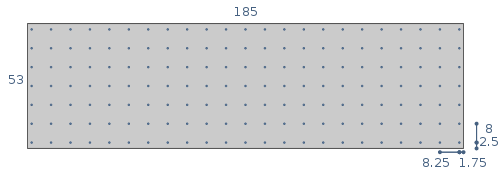
\includegraphics[width=.9\textwidth]{./figs/led_dist.png}
\caption{Led luminaires distributed along the facility ceiling.}
\label{fig:led_dist}
\end{figure}


\section{Calculus of Economy}

\subsection{Energy Consumption}
To calculate the energy consumption, the following data are needed:
\begin{itemize}
\item Number of luminaires: $161$
\item Energy cost: $0.093$\$
\item Electric demand cost: $11.00$\$
\item Number of hours per year: $16 \times 365.25 = 5,844$
\item Luminaire power: $310 W$
\end{itemize}
The numbers of hours per year assumes the leap year, so, the multiplier is $365.25$. The energy consumption results are showed as follow:
\begin{itemize}
\item Total power ($kW$): $161 \times 310 = 49,910 W = 49.91 kW$
\item Total electric demand cost per year: $11 \times 12 \times 49.91 = 6,588.12$\$
\item Total electric consumption cost per year: $5,844 \times 0.093 \times 49.91 = 27,125.69$\$
\item Total energy cost: $33,713.81$\$
\end{itemize}

\subsection{Average of Replaced Lamps per Year}
In order to calculate the average of lamps replaced per year, the following data are needed:
\begin{itemize}
\item Number of luminaires: $161$
\item Number of hours per year: $5,844$
\item Lamp lifetime hours at $80\%$ of survival: $60,000$
\end{itemize}

The Equation~\ref{eq:led_relamp_average} shows the replaced lamps calculus.

\begin{equation}
\begin{split}
 & \text{Individual replaced lamps} \\
M_{individual} & = 20\% \times 161 \times \frac{5,844}{60,000} \\
 & = 3.14 \\
 & \approx 4
\end{split}
\begin{split}
 & \text{Collective replaced lamps} \\
M_{collective} & = 161 \times \frac {5,844}{60,000} \\
 & = 15.68 \\
 & \approx 16
\end{split}
\label{eq:led_relamp_average}
\end{equation}
Taking into account the worst case scenario, the calculation for this average is ceiling rounded. Thus, the average of replaced lamps per year is $20$.

\subsection{Relamping Workforce Cost per Year}
In order to calculate the cost for the relamping workforce per year, the following data are needed:
\begin{itemize}
\item Average of individual lamps replaced per year: $4$
\item Individual relamping cost: $87.00$\$
\item Average of collective lamps replaced per year: $16$
\item Collective relamping cost: $9.00$\$
\end{itemize}
The average cost per year for the collective relamping is $144.00$\$ and for the individual relamping is $348,00$\$, so the total is $492,00$\$


